\chapterauthor{Bernd Krupinski}
\subsection{LineChart Control Implementierung}
Das LineChart Control wurde ähnlich die das Gauge Control ebenfalls mit 2 Canvas in einer Custom Control in WPF geschrieben. 1 Canvas für den Hintergrund und Skala und 1 Canvas für den Graphen selbst.\\
Das Control ist wie das GaugeControl ebenfalls stark anpassbar. Diese Werte sind unter anderen vertikale Linien zeichnen, horizontale Linien zeichnen, Anzahl horizontale/vertikale Linien, Füllfarbe, Strichfarbe und mehr funktionale Variablen wie Mindestwert, Maximalwert, Fenstergröße, Fensterposition.\\
Für die genaue Erklärungen für jeden Wert siehe in-Code Dokumentation.
Das Control nimmt eine Menge an Punkten an und versucht diese so gut wie möglich darzustellen. Dabei kann das Control nur ein Fenster (Siehe Variablen Fenstergröße, Fensterposition) oder die gesamte Menge anzeigen.\\
Dies geschieht wieder über ein Polygon. Allerdings muss darauf geachtet werden, dass das Canvas eine variable Größe hat. D.h. der Graph muss relativ gezeichnet werden. Es entstehen zwei Fälle:\\
\begin{itemize}
	\item Es existieren mehr Pixel als Sample
	\item Es existieren mehr Sample (Punkte) als Pixel
\end{itemize}
Diese werden im Code unterschieden.\\
\newpage
Für den Fall mehr Pixel als Sample, wird durch jedes Sample iteriert und berechnet wie viele Pixel das momentane Sample entspricht. In der Abbildung entspricht jedes Sample mit Abstand von drei, zwei Pixel.\\
\begin{figure}[ht]
	\centering
	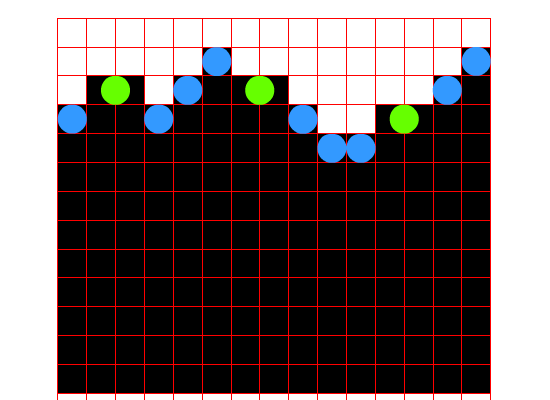
\includegraphics[width=0.6\textwidth]{TooFewSamples02}
	\caption{Beispiel: Mehr Pixel als Sample}
	\label{fig:gauge}
\end{figure}

Für den Fall mehr Sample als Pixel, wird wiederum durch jeden Pixel iteriert und berechnet welche Sample für das momentane Pixel relevant sind. Dabei werden stets 2 Pixel gleichzeitig betrachtet, da für die Darstellung das lokale Minimum und Maximum gezeichnet wird.\\

\begin{figure}[ht]
	\centering
	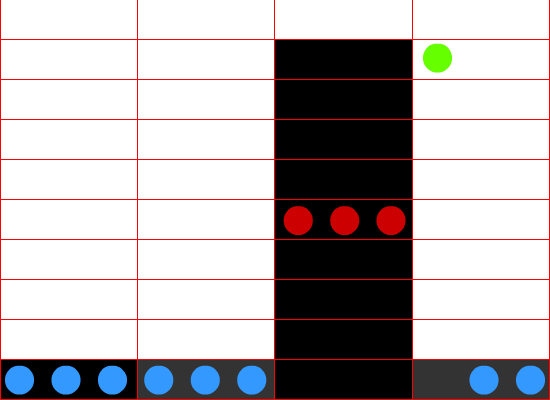
\includegraphics[width=0.6\textwidth]{TooManySamples030001}
	\caption{Beispiel: Mehr Pixel als Sample 01}
	\label{fig:gauge}
\end{figure}
In diese Abbildung zum Beispiel sind für die rechten zwei Pixel Spalten sechs Sample relevant. Drei rote Sample mit mittel hohen Wert, ein grünes Sample mit einem sehr hohen Wert und zwei blaue Sample mit niedrigen Werten.\\
Das Minimum und Maximum wird bestimmt. Das grüne Sample entspricht dem Maximum, während eins der blauen Sample das Mimimum entspricht. Da das Maximum (grün) rechts vom Minimum (blau) ist, wird entsprechend die linke Spalte das Maximum und die rechte Spalte das Minimum anzeigen.\\